	\section{Introduction}


    \begin{frame}{Introducing myself}
        \begin{columns}
            % Column 1
            \begin{column}{0.5\textwidth}
                \begin{itemize}
                    \item Isak Hammer, 27 year old, Lofoten
                    \item Graduate student in Industrial Mathematics
                    \item Research Focus: Analysis and numerical techniques for Partial Differential Equations (PDEs), with a strong emphasis on applications for Finite Element Methods (FEM).
                \end{itemize}
            \end{column}

            % Column 2
            \begin{column}{0.5\textwidth}
                \begin{figure}
                    \centering
                    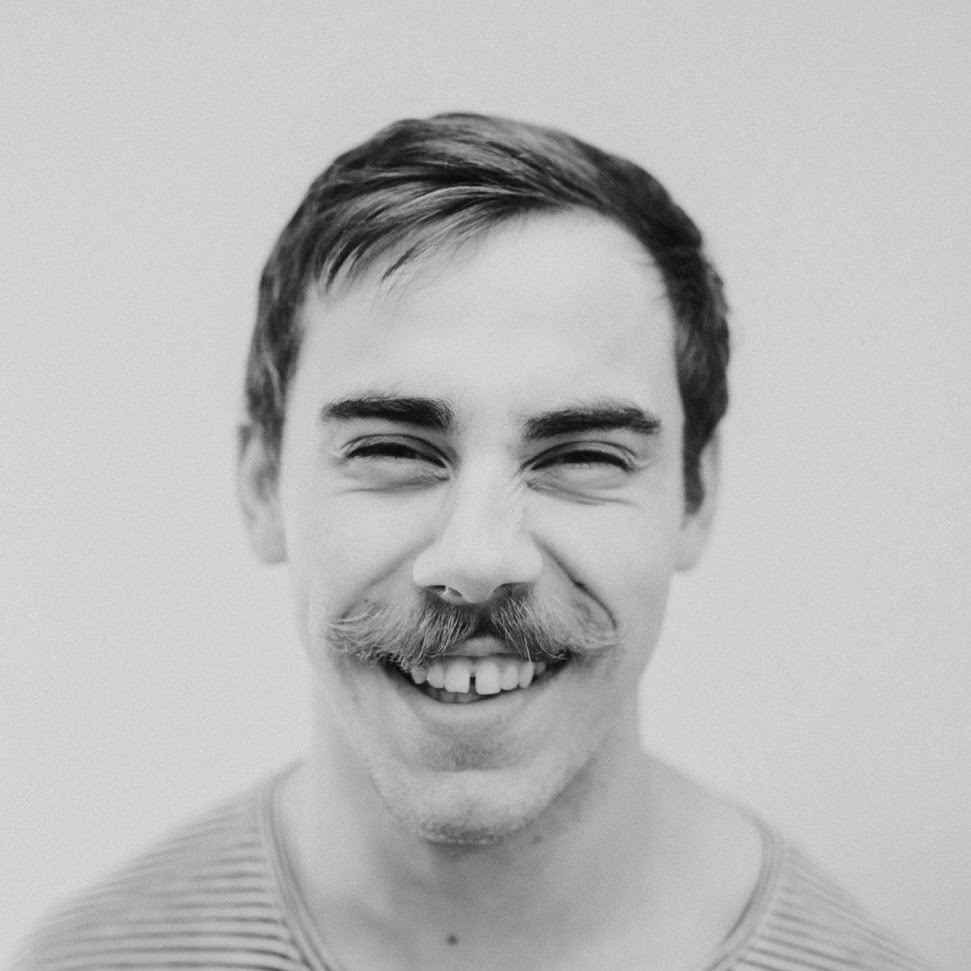
\includegraphics[width=0.7\textwidth]{figures/isak.jpg}
                \end{figure}
            \end{column}
        \end{columns}
    \end{frame}

\begin{frame}{Importance and Motivation of the Cahn Hilliard Equation}
    \begin{columns}
        % Column 1
        \begin{column}{0.5\textwidth}
            \begin{itemize}
                \item Thermodynamically modelling of a two-component liquid separation\footnotemark[1].
            \item Modelling of so-called lipid rafts in biological membrane dynamics \footnotemark[2].
            \end{itemize}
        \end{column}
        \begin{column}{0.5\textwidth}
            \begin{itemize}
                \item Droplet dynamics, i.e., coalescence, breakup and movement by coupling with Navier-Stokes \footnotemark[3].
            \end{itemize}
        \end{column}
    \end{columns}
    \footnotetext[1]{\fullcite{cahn1959free}}
    \footnotetext[2]{\fullcite{yushutin2019computational}}
    \footnotetext[3]{\fullcite{zimmermann2019calculation}}
\end{frame}

\begin{frame}
    \begin{block}{The Cahn Hilliard Equation}
        The general Cahn Hilliard Equation  has the form $u( t,x): \Omega \mapsto [-1,1]   $ s.t.
            \[
            \begin{split}
                 u_t+\Delta\left(\varepsilon \Delta u-\frac{1}{\varepsilon} f(u)\right)&=0 \quad \text{in } \Omega_T:=\Omega \times(0, T) \\
\partial_n u=\partial_n \Delta u& =0 \quad \text{on } \partial \Omega_T:=\partial \Omega \times(0, T) \\
 u & =u_0 \quad \text{on } \Omega \times\{0\}
            \end{split}
            \]
where $f(s)=F^{\prime}(s)$ and $F(s)=\frac{1}{4}\left(s^2-1\right)^2$ and $\Omega \subset \mathbf{R}^d, d=2,3$, is a bounded domain. $\partial_n$ denotes the normal derivative operator on $\partial \Omega$.
\end{block}

\begin{block}{Challenges}
    \begin{enumerate}
        \item Highly nonlinear and stiff. Often practical applications require $\varepsilon \ll 1$.
        \item 4th order system.
        \item Conservation of mass and the Neumann conditions conditions.
    \end{enumerate}
\end{block}

\end{frame}

\begin{frame}
    \begin{block}{Why Finite Element Method (FEM)}
        \begin{enumerate}
            \item \textbf{Flexibility:} Weak formulation provides versatility in imposing boundary conditions effectively.
            \item \textbf{Complex geometries:} FEM can efficiently handle intricate geometries, making it suitable for a wide range of applications.
            \item \textbf{Polynomial basis:} FEM is built upon polynomial basis functions, offering flexibility, accuracy and smoothness in the solution.
            \item \textbf{Other: } Elegant mathematical formulation, supports adaptive refinements, easily adaptable to multi-physics problems, among other benefits.
        \end{enumerate}
    \end{block}
\end{frame}

\begin{frame}
    \begin{block}{Strategy to solve the Cahn-Hilliard problem on smooth domains}
        \begin{enumerate}
            \item First find a suitable method to solve an 4th order PDE for polygonal domains.
            \item Modify the problem formulation to take account for smooth domains.
            \item Utilize the time integration to handle nonlinearity.
        \end{enumerate}
    \end{block}
\end{frame}

\begin{frame}
    \begin{block}{Strategy to solve the Cahn-Hilliard problem on smooth domains}
        \begin{enumerate}
            \item First find a suitable method to solve an 4th order PDE for polygonal domains.
            \item Modify the problem formulation to take account for smooth domains.
            \item Utilize the time integration to handle nonlinearity.
\item \textcolor{red}{Make the time-steps small enough or implement adaptivity time schemes.}
        \end{enumerate}
    \end{block}
\end{frame}


\begin{frame}
\begin{columns}
\column{0.55\textwidth}
\begin{block}{The Biharmonic Problem}
Let $\Omega \subseteq \mathbb{R} ^d$ be a bounded domain with boundary $\Gamma $ . Let the biharmonic problem have the form s.t. $u:\Omega \mapsto \mathbb{R} $,
\begin{equation}
\label{eq:bi_problem}
\begin{split}
\Delta^2 u + \alpha u & = f( x) \quad \text{in } \Omega, \\
\partial_{n} u & = g_{1} \quad \text{on } \Gamma , \\
\partial_{n} \Delta u & = g_{2} \quad \text{on } \Gamma . \\
\end{split}
\end{equation}
Here is $\Delta ^2 = \Delta \left( \Delta \right) $ the biharmonic operator. The functions $g_{1},g_{2}: \Omega \to \mathbb{R}$ are denoted as boundary conditions.
\end{block}

\column{0.45\textwidth}
\begin{figure}[htpb!]
    \centering
    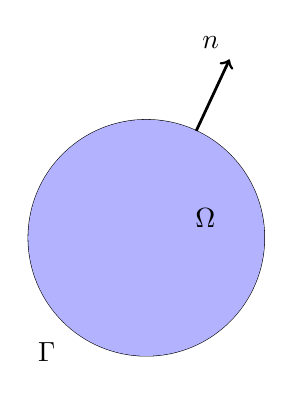
\begin{tikzpicture}
        % Circle
        \draw (0.0,0.0) circle (1.5cm);
        \fill[blue!30] (0.0,0.0) circle (1.5cm);

        \draw[->, line width=1.0pt] ({1.5*cos(65)}, { 1.5*sin(65) }) -- ({ 2.5*cos(65)  }, { 2.5*sin(65)  }) node[ above left] {$n $};
        % \draw[->, line width=1.0pt] ({1.5*cos(45)}, { 1.5*sin(45) }) -- ({ 1.5*cos(45) - 1.5*sin(45) }, { 1.5*sin(45) + 1.5*cos(45) }) node[ above right] {$t $};

        % Labels
        \node[below right] at (0.5,0.5) {$\Omega$};
        \node[below right] at (-1.5,-1.2) {$\Gamma$};
    \end{tikzpicture}
    \caption{ Illustration of the domain $\Omega $, the boundary $\Gamma $ and the normal vector $n$. }
    \label{fig:domain_construction}
\end{figure}
\end{columns}

\end{frame}

\begin{frame}
\begin{columns}
\column{0.55\textwidth}
\begin{block}{The Biharmonic Problem (on a mesh)}
    Let $\Omega \approx \Omega_{h} = \mathcal{T}_{h}$ be a bounded \textcolor{red}{polygonal} domain with boundary $\Gamma $ . Let the biharmonic problem have the form s.t. $u:\Omega \mapsto \mathbb{R} $,
\begin{equation}
\label{eq:bi_problem}
\begin{split}
\Delta^2 u + \alpha u & = f( x) \quad \text{in } \Omega, \\
\partial_{n} u & = 0 \quad \text{on } \Gamma , \\
\partial_{n} \Delta u & = 0 \quad \text{on } \Gamma . \\
\end{split}
\end{equation}
Here is $\Delta ^2 = \Delta \left( \Delta \right) $ the biharmonic operator. The functions $g_{1},g_{2}: \Omega_{h} \to \mathbb{R}$ are denoted as boundary conditions.
\end{block}

\column{0.45\textwidth}
\begin{figure}[htpb!]
    \centering
        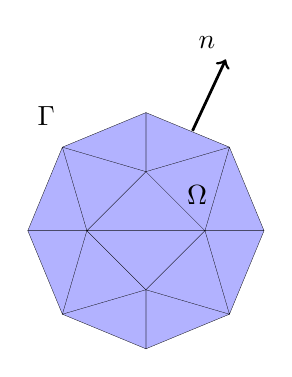
\begin{tikzpicture}
            % FIGURE OF FITTED MESH
            % Boundary points
            \foreach \i in {0, 45, ..., 315} {
                \coordinate (boundary-\i) at (\i:1.5cm);
            }
            % Interior points
            \coordinate (interior-1) at (0.75, 0);
            \coordinate (interior-2) at (-0.75, 0);
            \coordinate (interior-3) at (0, 0.75);
            \coordinate (interior-4) at (0, -0.75);

            % Create a cycle connecting all the boundary points
            \fill[blue!30] (boundary-0) -- (boundary-45) -- (boundary-90) -- (boundary-135) -- (boundary-180) -- (boundary-225) -- (boundary-270) -- (boundary-315) -- cycle;

            % Labels
            \node[below right] at (0.4,0.7) {$\Omega $};
            \node[below right] at (-1.5,1.7) {$\Gamma $};

            % Triangulation (manually specified)
            \draw[line width=0.1pt] (boundary-0) -- (boundary-45) -- (interior-1) -- cycle;
            \draw[line width=0.1pt] (boundary-45) -- (boundary-90) -- (interior-3) -- cycle;
            \draw[line width=0.1pt] (boundary-90) -- (boundary-135) -- (interior-3) -- cycle;
            \draw[line width=0.1pt] (boundary-135) -- (boundary-180) -- (interior-2) -- cycle;
            \draw[line width=0.1pt] (boundary-180) -- (boundary-225) -- (interior-2) -- cycle;
            \draw[line width=0.1pt] (boundary-225) -- (boundary-270) -- (interior-4) -- cycle;
            \draw[line width=0.1pt] (boundary-270) -- (boundary-315) -- (interior-4) -- cycle;
            \draw[line width=0.1pt] (boundary-315) -- (boundary-0) -- (interior-1) -- cycle;

            % Triangulation between interior points
            \draw[line width=0.1pt] (interior-1) -- (interior-2) -- (interior-3) -- cycle;
            \draw[line width=0.1pt] (interior-1) -- (interior-2) -- (interior-4) -- cycle;

            \draw[->, line width=1.0pt] ({1.4*cos(65)}, { 1.4*sin(65) }) -- ({ 2.4*cos(65)  }, { 2.4*sin(65)  }) node[ above left] {$n $};

        \end{tikzpicture}
    \caption{ Illustration of the mesh $\Omega_{h} $, the boundary $\Gamma $ and the normal vector $n$. }
    \label{fig:domain_construction}
\end{figure}
\end{columns}

\end{frame}


\begin{frame}
\begin{block}{Defining the global polynomial space}
    \begin{itemize}
        \item When writing the biharmonic on weak form we end up with Hessians/Laplacian.
        \item Thus, a requirement that solution is locally at least $\mathcal{P}^{k} $ for $k\ge 2$
        \item What should we require globally?
    \end{itemize}
\end{block}
\end{frame}

\begin{frame}

\begin{block}{Illustration the global $C^{1}$ continuous finite elements}
\begin{columns}

\begin{column}{0.3\textwidth}
    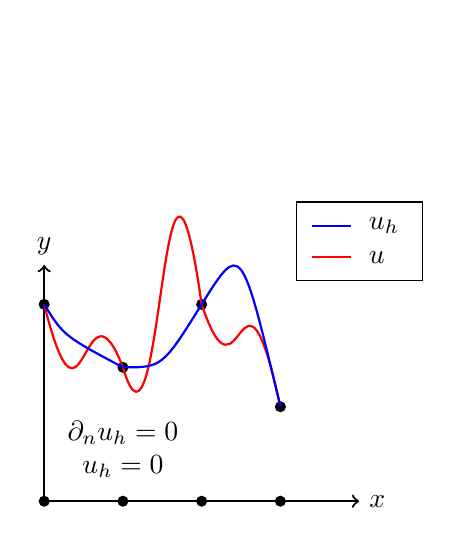
\begin{tikzpicture}
        % Draw x-axis
        \draw[->, thick] (0,0) -- (4,0) node[right] {$x$};
        % Draw y-axis
        \draw[->, thick] (0,0) -- (0,3) node[above] {$y$};

        % Draw nodes at center, A, B, and C with arbitrary y-values
        \foreach \x/\y in {0/2.5, 1/1.7, 2/2.5, 3/1.2} {
            \fill (\x,\y) circle (2pt); % Filled nodes with y-values
            \fill (\x,0) circle (2pt); % Filled circles on x-axis
        }

        % Exact solution
        \draw[red, thick] (0,2.5) .. controls (0.5,0.5) and (0.5,3) .. (1,1.7) .. controls (1.5,0) and (1.5,6) .. (2,2.5) .. controls (2.5,1) and (2.5,3.5) .. (3,1.2);
        \node at (1,0.6) [above] {$\jump{ \partial _{n} u_{h} } = 0$};
        \node at (1,0.7) [below] {$\jump{ u_{h} }   = 0$};

        % Second
        \draw[blue, thick]
        (0,2.5) .. controls (0.25,2.1) .. (1,1.7)
        (1,1.7) .. controls (1.5,1.7) .. (2,2.5)
        (2,2.5) .. controls (2.5,3.3) .. (3,1.2);

        \draw (3.2,2.8) rectangle (4.8,3.8); % Legend box
        \draw[blue, thick] (3.4,3.5) -- (3.9,3.5); % Blue line for u_h
        \draw[red, thick] (3.4,3.1) -- (3.9,3.1); % Red line for u
        \node[anchor=west] at (4.0,3.5) {$u_h$}; % Label for u_h
        \node[anchor=west] at (4.0,3.1) {$u$}; % Label for u
    \end{tikzpicture}
\end{column}

\begin{column}{0.5\textwidth}
    % Add your points here
    \begin{itemize}
        \item Let $\jump{ u_{h} } = u_{+} - u_{-} $ be defined as the jumps between elements.
        \item The numerical solution is \textbf{continuous}, i.e. $\jump{ u_{h} }     =0   $
        \item The numerical solution derivative is \textbf{continuous} , i.e. $\jump{ \partial _{n}u_{h} }     =0   $
        \item Not very flexible and difficult to implement in higher dimensions.\footnotemark[1]
    \end{itemize}
\end{column}
\footnotetext[1]{\fullcite{kapl2021family}}

\end{columns}
\end{block}
\end{frame}

\begin{frame}

\begin{block}{Illustration the global $C^{0}$ continuous $\mathcal{P}^k $  finite elements}
\begin{columns}
\begin{column}{0.3\textwidth}
    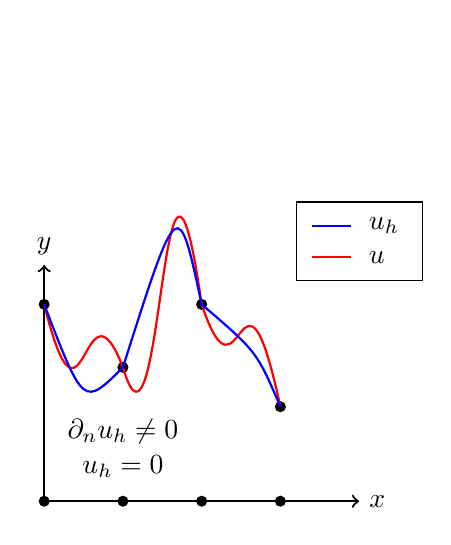
\begin{tikzpicture}
        % Draw x-axis
        \draw[->, thick] (0,0) -- (4,0) node[right] {$x$};
        % Draw y-axis
        \draw[->, thick] (0,0) -- (0,3) node[above] {$y$};

        % Draw nodes at center, A, B, and C with arbitrary y-values
        \foreach \x/\y in {0/2.5, 1/1.7, 2/2.5, 3/1.2} {
            \fill (\x,\y) circle (2pt); % Filled nodes with y-values
            \fill (\x,0) circle (2pt); % Filled circles on x-axis
        }

        % Exact solution
        \draw[red, thick] (0,2.5) .. controls (0.5,0.5) and (0.5,3) .. (1,1.7) .. controls (1.5,0) and (1.5,6) .. (2,2.5) .. controls (2.5,1) and (2.5,3.5) .. (3,1.2);
        \node at (1,0.6) [above] {$\jump{ \partial _{n} u_{h} } \neq 0$};
        \node at (1,0.7) [below] {$\jump{ u_{h} }   = 0$};

        %% Second
        \draw[blue, thick] (0,2.5) .. controls (0.5,1.2) .. (1,1.7)
        .. controls (1.7,3.9) .. (2,2.5)
        .. controls (2.7,1.9) .. (3,1.2); Second

        \draw (3.2,2.8) rectangle (4.8,3.8); % Legend box
        \draw[blue, thick] (3.4,3.5) -- (3.9,3.5); % Blue line for u_h
        \draw[red, thick] (3.4,3.1) -- (3.9,3.1); % Red line for u
        \node[anchor=west] at (4.0,3.5) {$u_h$}; % Label for u_h
        \node[anchor=west] at (4.0,3.1) {$u$}; % Label for u

    \end{tikzpicture}
\end{column}
\begin{column}{0.6\textwidth}
    % Add your points here
    \begin{itemize}
        \item Locally $\mathcal{P}^{k}( T)  $ of degree $k$, but globally $C^{0}$, i.e.,
            \[
            V_{h} = \left\{ v \in C^{0}\left( \Omega  \right): v_{T} = v | _{T} \in \mathcal{P} ^{k}\left( T \right), \forall T \in
\mathcal{T}_{h}    \right\}
            \]

        \item The numerical solution is \textbf{continuous} , i.e. $\jump{ u_{h} } = 0   $
        \item The numerical solution derivative is \textbf{discontinuous} , i.e. $\jump{ \partial _{n}u_{h} } \neq 0   $
    \end{itemize}
\end{column}
\end{columns}
\end{block}
\end{frame}

\begin{frame}
\frametitle{ $C^0$ Interior penalty method (CIP) }

\begin{block}{}
The discretized numerical problem is to solve $w \in V_{h}$ such that
\begin{equation*}
\label{eq:CP_A_F}
a_{h}( w, v )   = l_{h}( v), \quad \forall v \in V_{h}  .
\end{equation*}
where

\begin{equation*}
\begin{split}
a_{h} \left( w, v \right)   =&
    \left( \alpha  w, v \right) _{\Omega }   +  \left( \Delta  w, \Delta v \right) _{\mathcal{T} _{h}} \\
 & +
  \left( \mean{  \Delta  w }, \jump{ \partial _{n }v} \right)_{\mathcal{F}_{h}}  +
 \left( \mean{ \Delta  v }, \jump{ \partial _{n}w }      \right)_{\mathcal{F}_{h}}  + \frac{\gamma }{h}  \left( \jump{ \partial _{n} w}, \jump{ \partial _{n} v   }   \right)_{\mathcal{F}_{h}} \\
 l_{h}( v_{h}) & =  \left( f, v \right) _{\Omega }
\end{split}
\end{equation*}

Which is inspired from Brenner2012 \footnotemark[1]
\end{block}

\footnotetext[1]{\fullcite{brenner2012}}

\end{frame}

\begin{frame}
\frametitle{Cut Finite Element Method (CutFEM)}

\begin{block}{Unfitted mesh vs fitted mesh}
    CutFEM is a numerical method for solving partial differential equations (PDEs) using an unfitted mesh.

\begin{figure}
    \centering
    % First TikZ picture
    \begin{minipage}{0.45\textwidth}
        \centering
        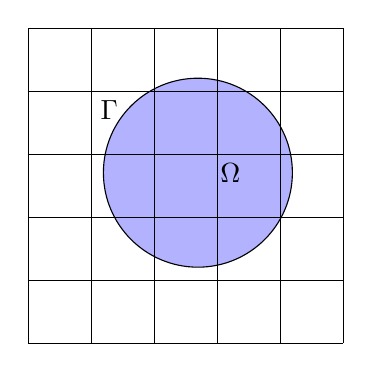
\begin{tikzpicture}[scale=0.80]
            \draw[fill=blue!30] (0.2, 0.2) circle (1.5cm);
            % Background mesh
            \foreach \i in {-2.5, -1.5, ..., 2.5} {
                \draw[line width=0.1pt, shift={(-2.5,\i)}] (0,0) -- (5,0);
                \draw[line width=0.1pt, shift={(\i,-2.5)}] (0,0) -- (0,5);
            }
            % Labels
            \node[below right] at (0.4,0.5) {$\Omega $};
            \node[below right] at (-1.5,1.5) {$\Gamma $};
            % \draw[blue, thick] (-2.5, -2.5) rectangle (2.5, 2.5);
        \end{tikzpicture}
    \end{minipage}
    \hfill
    % Second TikZ picture
    \begin{minipage}{0.45\textwidth}
        \centering
        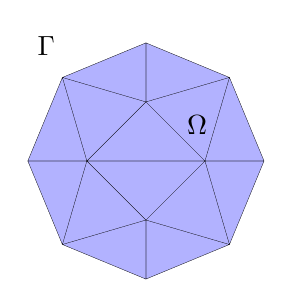
\begin{tikzpicture}[scale=1.0]
            % FIGURE OF UNFITTED MESH
            % Boundary points
            \foreach \i in {0, 45, ..., 315} {
                \coordinate (boundary-\i) at (\i:1.5cm);
            }
            % Interior points
            \coordinate (interior-1) at (0.75, 0);
            \coordinate (interior-2) at (-0.75, 0);
            \coordinate (interior-3) at (0, 0.75);
            \coordinate (interior-4) at (0, -0.75);

            % Create a cycle connecting all the boundary points
            \fill[blue!30] (boundary-0) -- (boundary-45) -- (boundary-90) -- (boundary-135) -- (boundary-180) -- (boundary-225) -- (boundary-270) -- (boundary-315) -- cycle;

            % Labels
            \node[below right] at (0.4,0.7) {$\Omega $};
            \node[below right] at (-1.5,1.7) {$\Gamma $};

            % Triangulation (manually specified)
            \draw[line width=0.1pt] (boundary-0) -- (boundary-45) -- (interior-1) -- cycle;
            \draw[line width=0.1pt] (boundary-45) -- (boundary-90) -- (interior-3) -- cycle;
            \draw[line width=0.1pt] (boundary-90) -- (boundary-135) -- (interior-3) -- cycle;
            \draw[line width=0.1pt] (boundary-135) -- (boundary-180) -- (interior-2) -- cycle;
            \draw[line width=0.1pt] (boundary-180) -- (boundary-225) -- (interior-2) -- cycle;
            \draw[line width=0.1pt] (boundary-225) -- (boundary-270) -- (interior-4) -- cycle;
            \draw[line width=0.1pt] (boundary-270) -- (boundary-315) -- (interior-4) -- cycle;
            \draw[line width=0.1pt] (boundary-315) -- (boundary-0) -- (interior-1) -- cycle;

            % Triangulation between interior points
            \draw[line width=0.1pt] (interior-1) -- (interior-2) -- (interior-3) -- cycle;
            \draw[line width=0.1pt] (interior-1) -- (interior-2) -- (interior-4) -- cycle;

            % \draw[blue, thick] (-2.5, -2.5) rectangle (2.5, 2.5);

        \end{tikzpicture}
    \end{minipage}


    % \caption{Mesh comparison: unfitted mesh (left) adheres to domain and boundary, while fitted mesh (right) employs a triangular mesh for polygonal approximation of the circular domain.}
    \label{fig:domain_mesh}
    \end{figure}
\end{block}

\end{frame}


\begin{frame}
\frametitle{Cut Finite Element Method (CutFEM)}

A recent and promising numerical technique for PDEs, has gained significant momentum in the past decade \footnotemark[1]\footnotemark[2].

\begin{block}{}
    \begin{itemize}
        \item  Can handle smooth boundaries $\Gamma \in C^2 $, very complex domains and moving domains efficiently.
        \item Utilizing so-called ghost penalties to ensure well-posedness on the so-called cut cells.
        \item Diving the computational domains into background, active and interior mesh.
    \end{itemize}
\end{block}
\footnotetext[1]{\fullcite{burman2015cutfem}}
\footnotetext[2]{\fullcite{gurkan2019stabilized}}

\end{frame}

\begin{frame}
    \frametitle{Cut Finite Element method}
Background Mesh
    \begin{block}{}
        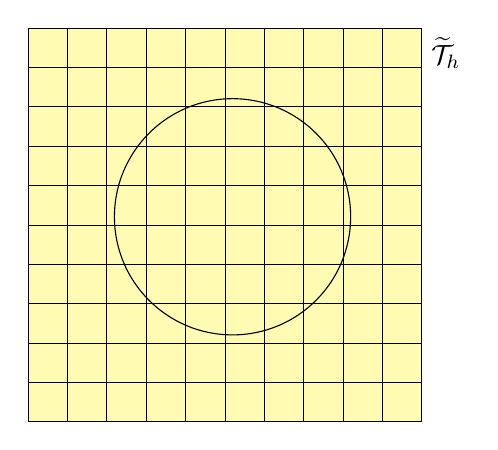
\begin{tikzpicture}[scale=1.0]

            \fill[yellow!30] (-2.5,2.5) -- (2.5,2.5) -- (2.5,-2.5) -- (-2.5,-2.5) -- cycle;

            \draw (0.1, 0.1) circle (1.5cm);
            % Background mesh
            \foreach \i in {-2.5, -2, ..., 2.5} {
                \draw[line width=0.1pt, shift={(-2.5,\i)}] (0,0) -- (5,0);
                \draw[line width=0.1pt, shift={(\i,-2.5)}] (0,0) -- (0,5);
            }


            % Labels
            \node[below right] at (2.5,2.5) {$\widetilde{\mathcal{T}}_{h}$};
        \end{tikzpicture}
    \end{block}
\end{frame}

\begin{frame}
    \frametitle{Cut Finite Element method}
    Active Mesh
    \begin{block}{}
        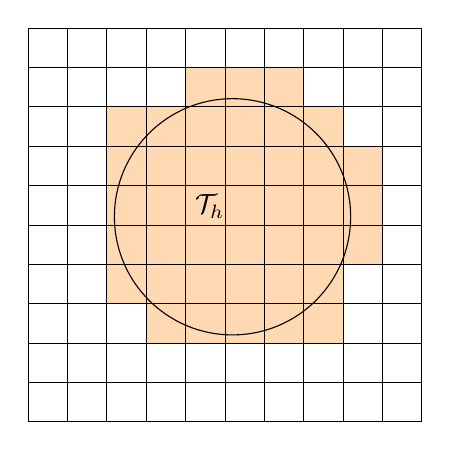
\begin{tikzpicture}[scale=1.0]

            % POTENTIAL ACTIVE MESH
            \fill[orange!30] (2,2) -- (2,-1.5) --(-1.5,-1.5) -- (-1.5,2) -- cycle;

            % ELEMENTS WITH NO INTERSECTION
            % lower left
            \fill[white] (-1.5,-1.5) rectangle (-1.0,-1.0);
            \fill[white] (-1.5,2.0) rectangle (-1.0,1.5);
            \fill[white] (-1.0,2.0) rectangle (-0.5,1.5);
            \fill[white] (2,2) rectangle (1.5,1.5);
            \fill[white] (1.5,2) rectangle (1.0,1.5);
            \fill[white] (2,1.5) rectangle (1.5,1.0);
            \fill[white] (1.5,-1) rectangle (2,-1.5);
            \fill[white] (1.5,-0.5) rectangle (2,-1.0);

            % CUT ELEMENTS
            \fill[orange!30] (-0.5,2.0) rectangle (1.0,1.5);
            \fill[orange!30] (-1.5,1.5) rectangle (0.0,1.0);
            \fill[orange!30] (0.5,1.5) rectangle (1.5,1.0);
            \fill[orange!30] (-1.5,1.0) rectangle (-1.0,-1.0);
            \fill[orange!30] (-1.0,-0.5) rectangle (-0.5,-1.5);
            \fill[orange!30] (-0.5,-1.5) rectangle (1.5,-1.0);
            \fill[orange!30] (1.5,-1) rectangle (1.0,-0.0);
            \fill[orange!30] (1.5,-0.5) rectangle (2.0,1.0);
            \fill[orange!30] (1.0,0.5) rectangle (1.5,1.0);

            \draw (0.1, 0.1) circle (1.5cm);
            % Background mesh
            \foreach \i in {-2.5, -2, ..., 2.5} {
                \draw[line width=0.1pt, shift={(-2.5,\i)}] (0,0) -- (5,0);
                \draw[line width=0.1pt, shift={(\i,-2.5)}] (0,0) -- (0,5);
            }


            % Labels
            % \node[below right] at (2.5,2.5) {$\widetilde{\mathcal{T}}_{h}$};
            % \node[below right] at (0.4,0.5) {$\mathcal{T}_{int}$};
            \node[below right] at (-0.5,0.5) {$\mathcal{T}_{h }$};
        \end{tikzpicture}
    \end{block}
\end{frame}

\begin{frame}
    \frametitle{Cut Finite Element method}
    Interior mesh and Cut Cells
    \begin{block}{}
        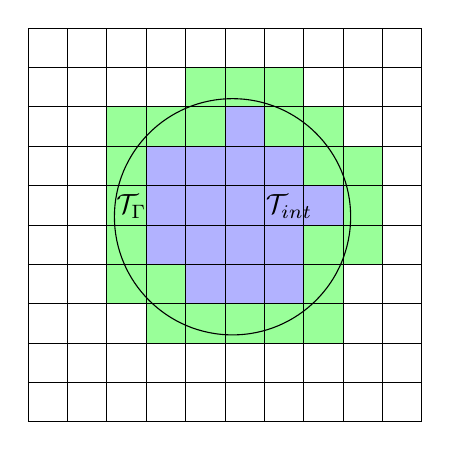
\begin{tikzpicture}[scale=1]

            % POTENTIAL ACTIVE MESH
            \fill[blue!30] (2,2) -- (2,-1.5) --(-1.5,-1.5) -- (-1.5,2) -- cycle;

            % ELEMENTS WITH NO INTERSECTION
            % lower left
            \fill[white] (-1.5,-1.5) rectangle (-1.0,-1.0);
            \fill[white] (-1.5,2.0) rectangle (-1.0,1.5);
            \fill[white] (-1.0,2.0) rectangle (-0.5,1.5);
            \fill[white] (2,2) rectangle (1.5,1.5);
            \fill[white] (1.5,2) rectangle (1.0,1.5);
            \fill[white] (2,1.5) rectangle (1.5,1.0);
            \fill[white] (1.5,-1) rectangle (2,-1.5);
            \fill[white] (1.5,-0.5) rectangle (2,-1.0);

            % CUT ELEMENTS
            \fill[green!40] (-0.5,2.0) rectangle (1.0,1.5);
            \fill[green!40] (-1.5,1.5) rectangle (0.0,1.0);
            \fill[green!40] (0.5,1.5) rectangle (1.5,1.0);
            \fill[green!40] (-1.5,1.0) rectangle (-1.0,-1.0);
            \fill[green!40] (-1.0,-0.5) rectangle (-0.5,-1.5);
            \fill[green!40] (-0.5,-1.5) rectangle (1.5,-1.0);
            \fill[green!40] (1.5,-1) rectangle (1.0,-0.0);
            \fill[green!40] (1.5,-0.5) rectangle (2.0,1.0);
            \fill[green!40] (1.0,0.5) rectangle (1.5,1.0);

            \draw (0.1, 0.1) circle (1.5cm);
            % Background mesh
            \foreach \i in {-2.5, -2, ..., 2.5} {
                \draw[line width=0.1pt, shift={(-2.5,\i)}] (0,0) -- (5,0);
                \draw[line width=0.1pt, shift={(\i,-2.5)}] (0,0) -- (0,5);
            }


            % Labels
            \node[below right] at (0.4,0.5) {$\mathcal{T}_{int}$};
            \node[below right] at (-1.5,0.5) {$\mathcal{T}_{\Gamma }$};
        \end{tikzpicture}
    \end{block}
\end{frame}



\begin{frame}
\frametitle{ Cut $C^0$ Interior penalty method (CutCIP) }

\begin{block}{}
The discretized numerical problem is to solve $w \in V_{h}$ such that
\begin{equation*}
\label{eq:CP_A_F}
A( w, v )  = a_{h}( w,v) + \textcolor{red}{g_{h}( w,v)}  = l_{h}( v), \quad \forall v \in V_{h}  .
\end{equation*}

Where the additional bilinear term $g_{h}( w,v) : V_{h} \times V_{h} \to  \mathbb{R} $ is the so-called \textbf{ghost penalty}, which does the numerical regularization.

\end{block}

\end{frame}
